\documentclass[a4paper, 10pt]{article}
\hyphenpenalty=8000
\textwidth=125mm
\textheight=185mm

\usepackage{graphicx}
%this package is flexible for image insertion
%
\usepackage{alltt}
%this package is suitable for the description of algorithms and computer programs
%
\usepackage{amsmath}
%this package draws mathematical symbols smoothly
%
\usepackage[hidelinks, pdftex]{hyperref}
%this package produces hypertext links in the document

\pagenumbering{arabic}
\setcounter{page}{1}
\renewcommand{\thefootnote}{\fnsymbol{footnote}}
\newcommand{\doi}[1]{\href{https://doi.org/#1}{\texttt{https://doi.org/#1}}}

\begin{document}

\begin{center}
Nonlinear Analysis: Modelling and Control, Vol. vv, No. 03, 2025\\
\copyright\ IE Infotep\\[24pt]
\LARGE
\textbf{Análisis con Kmeans}\\[6pt]
\small
\textbf {Diego Alzate, Aris Avila, Julieth Gutierrez}\\[6pt]
\end{center}

\begin{abstract}
Este informe presenta un estudio sobre la vulnerabilidad de los diferentes grupos de edad frente al COVID-19, teniendo como referencia la siguiente pregunta: ¿Que grupo de edad es mas vulnerable a verse afectado por el COVID-19?. El enfoque se basa en agrupar a las personas en tres grupos de edad y analizar cómo se distribuyen en función de la edad y el sexo. Para este análisis vamos a utilizar el algoritmo K-Means compartido por el profesor en clase.\\

\textbf{Palabras clave:} Grupos de edad, vulnerabilidad, COVID-19, K-Means, análisis de datos.
\end{abstract}

\section{Introducción}\label{s:1}
Sabemos que el COVID-19 afecto a millones de personas, sin importarle grupos de edad o sexo. En este trabajo, se utiliza el algoritmo K-Means para agrupar los datos de edad y sexo de una base de datos en excel compartida por el profesor y analizar para conseguir los grupos de edad más vulnerables.

\section{Cómo se realizó el trabajo}\label{s:2}
En este estudio, se tomó un conjunto de datos, donde se organizaron y se seleccionaron las columnas de Edad y Sexo. 

La Edad fue normalizada en tres categorías de la siguiente manera:

\begin{itemize}
    \item \textbf{1 a 20 años} (Grupo 1)
    \item \textbf{21 a 40 años} (Grupo 2)
    \item \textbf{41 años o más} (Grupo 3)
\end{itemize}

En cuanto al Sexo, se asignaron los siguientes valores:

\begin{itemize}
    \item \textbf{0} = Masculino
    \item \textbf{1} = Femenino
\end{itemize}

Luego de tener ambos campos normalizados, se realizó una función que recibe como parámetros la ruta del archivo y la cantidad de registros que se van a tomar por muestra. Esto se hace para optimizar el proceso de lectura, dado que la base de datos es muy grande, permitiendo así obtener resultados rápidamente. 

\subsection{Función para generar la matriz 2D}\label{s:2.2}

La siguiente función carga una cantidad específica de muestras del archivo y genera la matriz 2D con los datos de Edad Normalizada y Sexo:

\begin{alltt}
def generar_matriz_2d(file_path, n_samples=1000):
    """
    Genera una matriz 2D tomando una cantidad específica de muestras del archivo.

    Parametros:
        file_path (str): Ruta del archivo CSV.
        n_samples (int): Cantidad de muestras a leer del archivo.

    Retorna:
        matriz_2d (numpy.ndarray): Matriz 2D generada con Edad_Normalizada y Sexo.
    """

    # Cargar solo las primeras 'n_samples' filas del archivo
    df = pd.read_csv(file_path, encoding="latin1", sep=";", low_memory=False, nrows=n_samples)

    # Verificar que las columnas "Edad_Normalizada" y "Sexo" existen
    if "Edad_Normalizada" in df.columns and "Sexo" in df.columns:

        # Convertir la columna "Sexo" a valores numéricos (M=0, F=1)
        df['Sexo_Num'] = df['Sexo'].map({'M': 0, 'F': 1})

        # Obtener los valores de Edad_Normalizada y Sexo_Num
        edad_normalizada = df["Edad_Normalizada"].values
        sexo_num = df["Sexo_Num"].values

        # Crear la matriz 2D
        matriz_2d = np.column_stack((edad_normalizada, sexo_num))

        # Mostrar la matriz generada
        print(matriz_2d)
        
        return matriz_2d
    else:
        print("Las columnas 'Edad_Normalizada' y/o 'Sexo' no se encontraron en el archivo.")
        return None 
\end{alltt}

Esta función carga un número específico de muestras del archivo, convierte la columna de Sexo en valores numéricos (0 para masculino y 1 para femenino), y luego crea la matriz 2D combinando Edad Normalizada y Sexo. Posteriormente, esta matriz es utilizada para el análisis de agrupamiento mediante el algoritmo K-Means.


\subsection{Ejemplo de código para la generación de los datos y el gráfico}\label{s:2.1}

El siguiente código muestra cómo se cargan los datos y cómo se aplica el algoritmo K-Means para obtener los grupos de edad:

\begin{alltt}
file_path = "archivo_normalizado.csv"  # Ruta del archivo
n_samples = 2000  #cantidad de registros a tomar del archivo 
matriz_2d = generar_matriz_2d(file_path, n_samples)

# Aplicar K-Means
points = matriz_2d
kmeans = KMeans(k=3)
labels = kmeans.run(points)
print(labels)
print(kmeans.centroids)

# Generar el gráfico 2D
dibujar2D(points, kmeans.centroids, labels)
\end{alltt}

Este código permite cargar una muestra de los datos, aplicar el algoritmo K-Means, y generar un gráfico 2D de la distribución de los puntos antes y después del agrupamiento.

\subsection{resultados de  la Gráfico 2D}\label{s:3.2}

Se muestra el gráfico de los puntos antes y después de aplicar el algoritmo K-Means. Los puntos están coloreados según el grupo al que fueron asignados por el algoritmo.

\begin{figure}[ht]
\centering
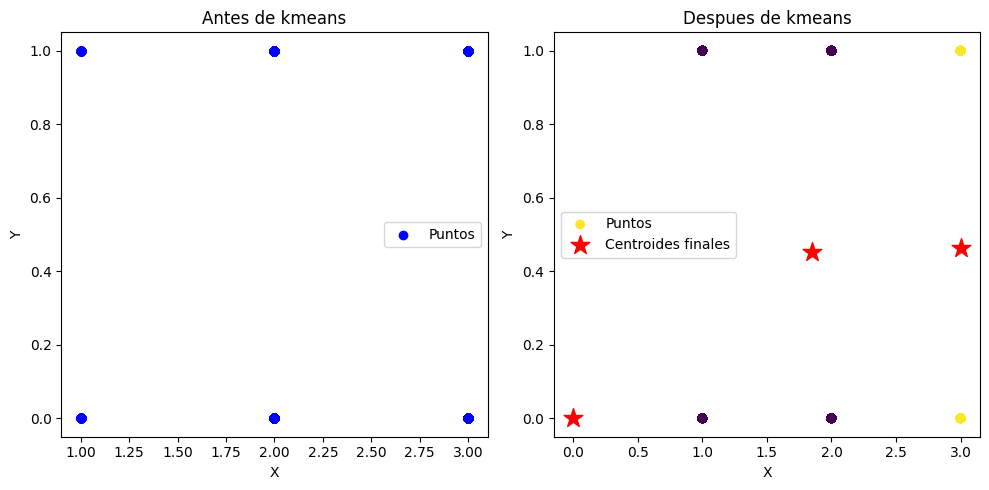
\includegraphics[width=0.8\textwidth]{resultado.png}  % Asegúrate de que la imagen esté en el mismo directorio
\caption{Gráfico 2D mostrando los puntos antes y después de aplicar K-Means, con centroides marcados.}
\end{figure}

\section{Conclusión}\label{s:4}
Al analizar el gráfico generado, podemos observar que los puntos de datos están ubicados casi en una única línea, lo que da la impresión de que solo hay un punto por opción de resultado. Esta distribución no nos permite realizar un análisis correcto.

Además, concluimos que este enfoque, basado únicamente en Edad Normalizada y Sexo, no es la mejor manera de abordar este análisis. La visualización y los resultados sugieren que se necesitan más variables u otra manera de realizar el estudio.

\end{document}